\documentclass[10pt, a4paper]{article} % 设置字体大小和纸张类型
\usepackage{booktabs} % 支持更专业的表格线条
\usepackage{ctex}
\usepackage{caption} % 插图和表格的标题格式
\usepackage{amsmath, amsfonts, amssymb} % 数学公式支持
\usepackage{graphicx} % 插入图片
\usepackage{hyperref} % 超链接支持
\usepackage{geometry}
\usepackage{titlesec}
\usepackage{fmtcount} % 用于数字到中文的转换
\usepackage{enumitem} % 加载 enumitem 宏包
\usepackage{multirow} % 支持多行单元格
\usepackage{diagbox}
\geometry{a4paper, margin=1.5cm} % 设置页边距

% \renewcommand{\thesection}{\chinese{section}、}
% \renewcommand{\thesubsection}{\arabic{subsection}.}

\title{电子电路基础第二次研讨内容}
\author{朱海心 2024270901003 吕俊霆 2024270901009}
\date{\today}


\begin{document}

\maketitle

\section{场效应管的特性仿真}

仿真电路如图所示, 仿真分析N沟道增强型MOSFET的电压-电流关系曲线。(场效应管可以选择2N7000, 画图最好能采用MATLAB)

\begin{figure}[ht]
    \centering
    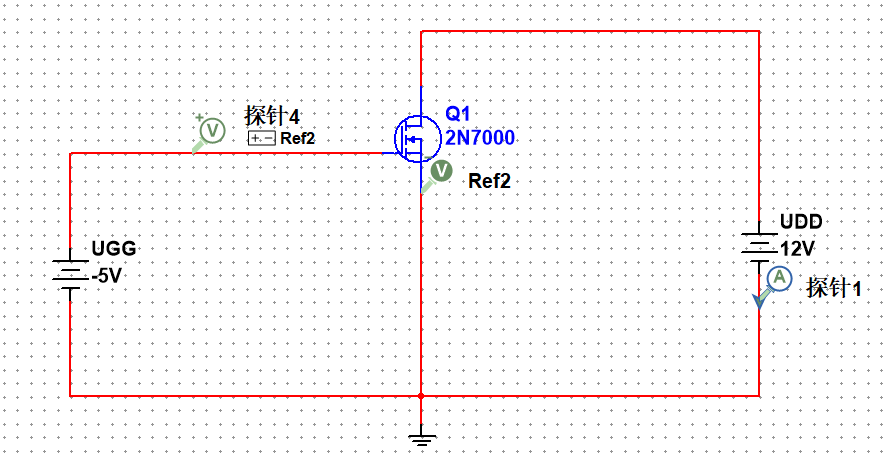
\includegraphics[width=0.7\linewidth]{image/1.png}
    \label{a}
\end{figure}

(1)固定$U_{DD}$ = 12V, 完成下列数据测试, 并画出$I_D$和$U_{GS}$的关系。

\begin{table}[htbp]
    \centering
    \label{tab:a}
    \begin{tabular}{|c|c|c|c|}
    \hline
    $U_{DD}(V)$&$U_{GG}(V)$&$U_{GS}(V)$&$I_{D}(mA)$\\
    12&-5 &-5 &0    \\ \hline
    12&-4 &-4 &0    \\ \hline
    12&-3 &-3 &0    \\ \hline
    12&-2 &-2 &0    \\ \hline
    12&-1 &-1 &0    \\ \hline
    12&0  &0  &0    \\ \hline
    12&1  &1  &0    \\ \hline
    12&1.5&1.5&0    \\ \hline
    12&2  &2  &0    \\ \hline
    12&2.5&2.5&-0.01\\ \hline
    12&3  &3  &-0.05\\ \hline
    12&3.5&3.5&-0.11\\ \hline
    12&4  &4  &-0.20\\ \hline
    12&4.5&4.5&-0.31\\ \hline
    12&5  &5  &-0.45\\ \hline
    12&6  &6  &-0.80\\ \hline
    12&7  &7  &-1.24\\ \hline
    12&8  &8  &-1.79\\
    \hline
    \end{tabular}
\end{table}

\newpage

\begin{figure}[htbp]
    \centering
    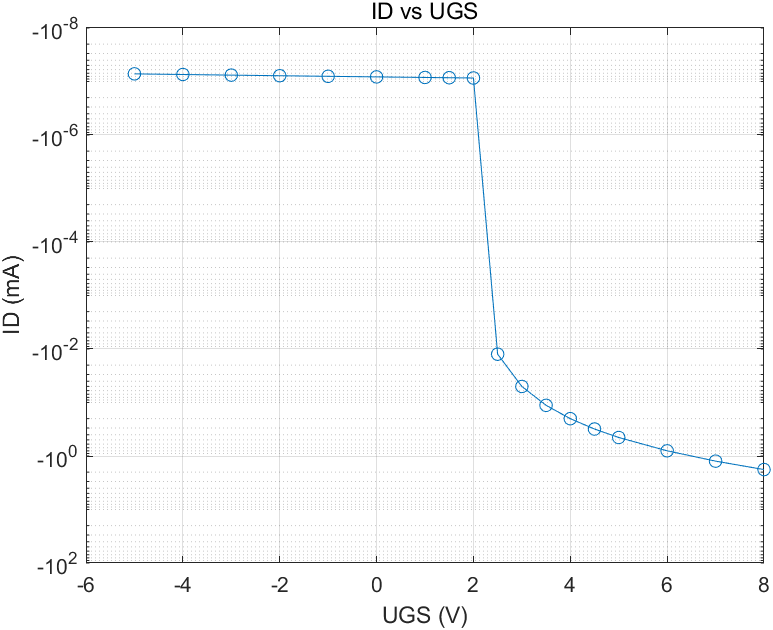
\includegraphics[width=0.8\linewidth]{image/5.png}
    \caption{Id-Ugs关系曲线}
    \label{fig:Id-Ugs}
\end{figure}

(2)测试在不同$U_{GG}$、$U_{DD}$作用下的$I_{D}$和$U_{DS}$, 并画出$I_{D}$和$U_{DS}$的关系

\begin{table}[ht]
    \centering
    \label{tab:b}
    \begin{tabular}{|c|c|c|c|c|}
        \hline
        $U_{GG}(V)$&$U_{DD}(V)$&$U_{GS}(V)$&$U_{DS}(V)$&$I_{D}(mA)$\\ \hline
        \multirow{12}{*}{2} &0  &2 &0  &2e-12  \\ \cline{2-5}
                            &0.5&2 &0.5&6e-12  \\ \cline{2-5}
                            &1  &2 &1  &1e-11  \\ \cline{2-5}
                            &1.5&2 &1.5&1.4e-11\\ \cline{2-5}
                            &2  &2 &2  &1.8e-11\\ \cline{2-5}
                            &2.5&2 &2.5&2.2e-11\\ \cline{2-5}
                            &3  &2 &3  &2.6e-11\\ \cline{2-5}
                            &4  &2 &4  &3.4e-11\\ \cline{2-5}
                            &6  &2 &6  &5.0e-11\\ \cline{2-5}
                            &8  &2 &8  &6.3e-11\\ \cline{2-5}
                            &10 &2 &10 &7.5e-11\\ \cline{2-5}
                            &12 &2 &12 &8.7e-11\\ \hline
        \multirow{12}{*}{3} &0  &3 &0  &35 \\ \cline{2-5} 
                            &0.5&3 &0.5&50 \\ \cline{2-5}
                            &1  &3 &1  &50 \\ \cline{2-5}
                            &1.5&3 &1.5&50 \\ \cline{2-5}
                            &2  &3 &2  &50 \\ \cline{2-5}
                            &2.5&3 &2.5&50 \\ \cline{2-5}
                            &3  &3 &3  &50 \\ \cline{2-5}
                            &4  &3 &4  &50 \\ \cline{2-5}
                            &6  &3 &5  &50 \\ \cline{2-5}
                            &8  &3 &6  &50 \\ \cline{2-5}
                            &10 &3 &8  &50 \\ \cline{2-5}
                            &12 &3 &10 &50 \\ \hline
    \end{tabular}
\end{table}

\begin{figure}[ht]
    \centering
    \begin{minipage}[ht]{0.48\linewidth}
        \centering
        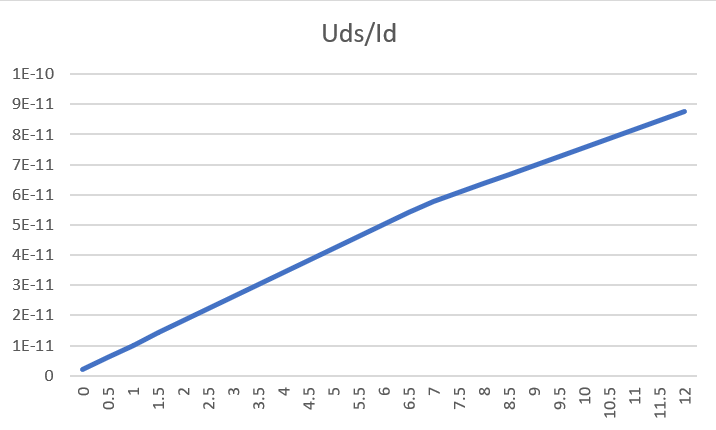
\includegraphics[width=\linewidth]{image/6.png}
        \caption{Id-Uds关系曲线(Ugg=2V)}
        \label{fig:Id-Uds1}
    \end{minipage}
    \hfill
    \begin{minipage}[ht]{0.48\linewidth}
        \centering
        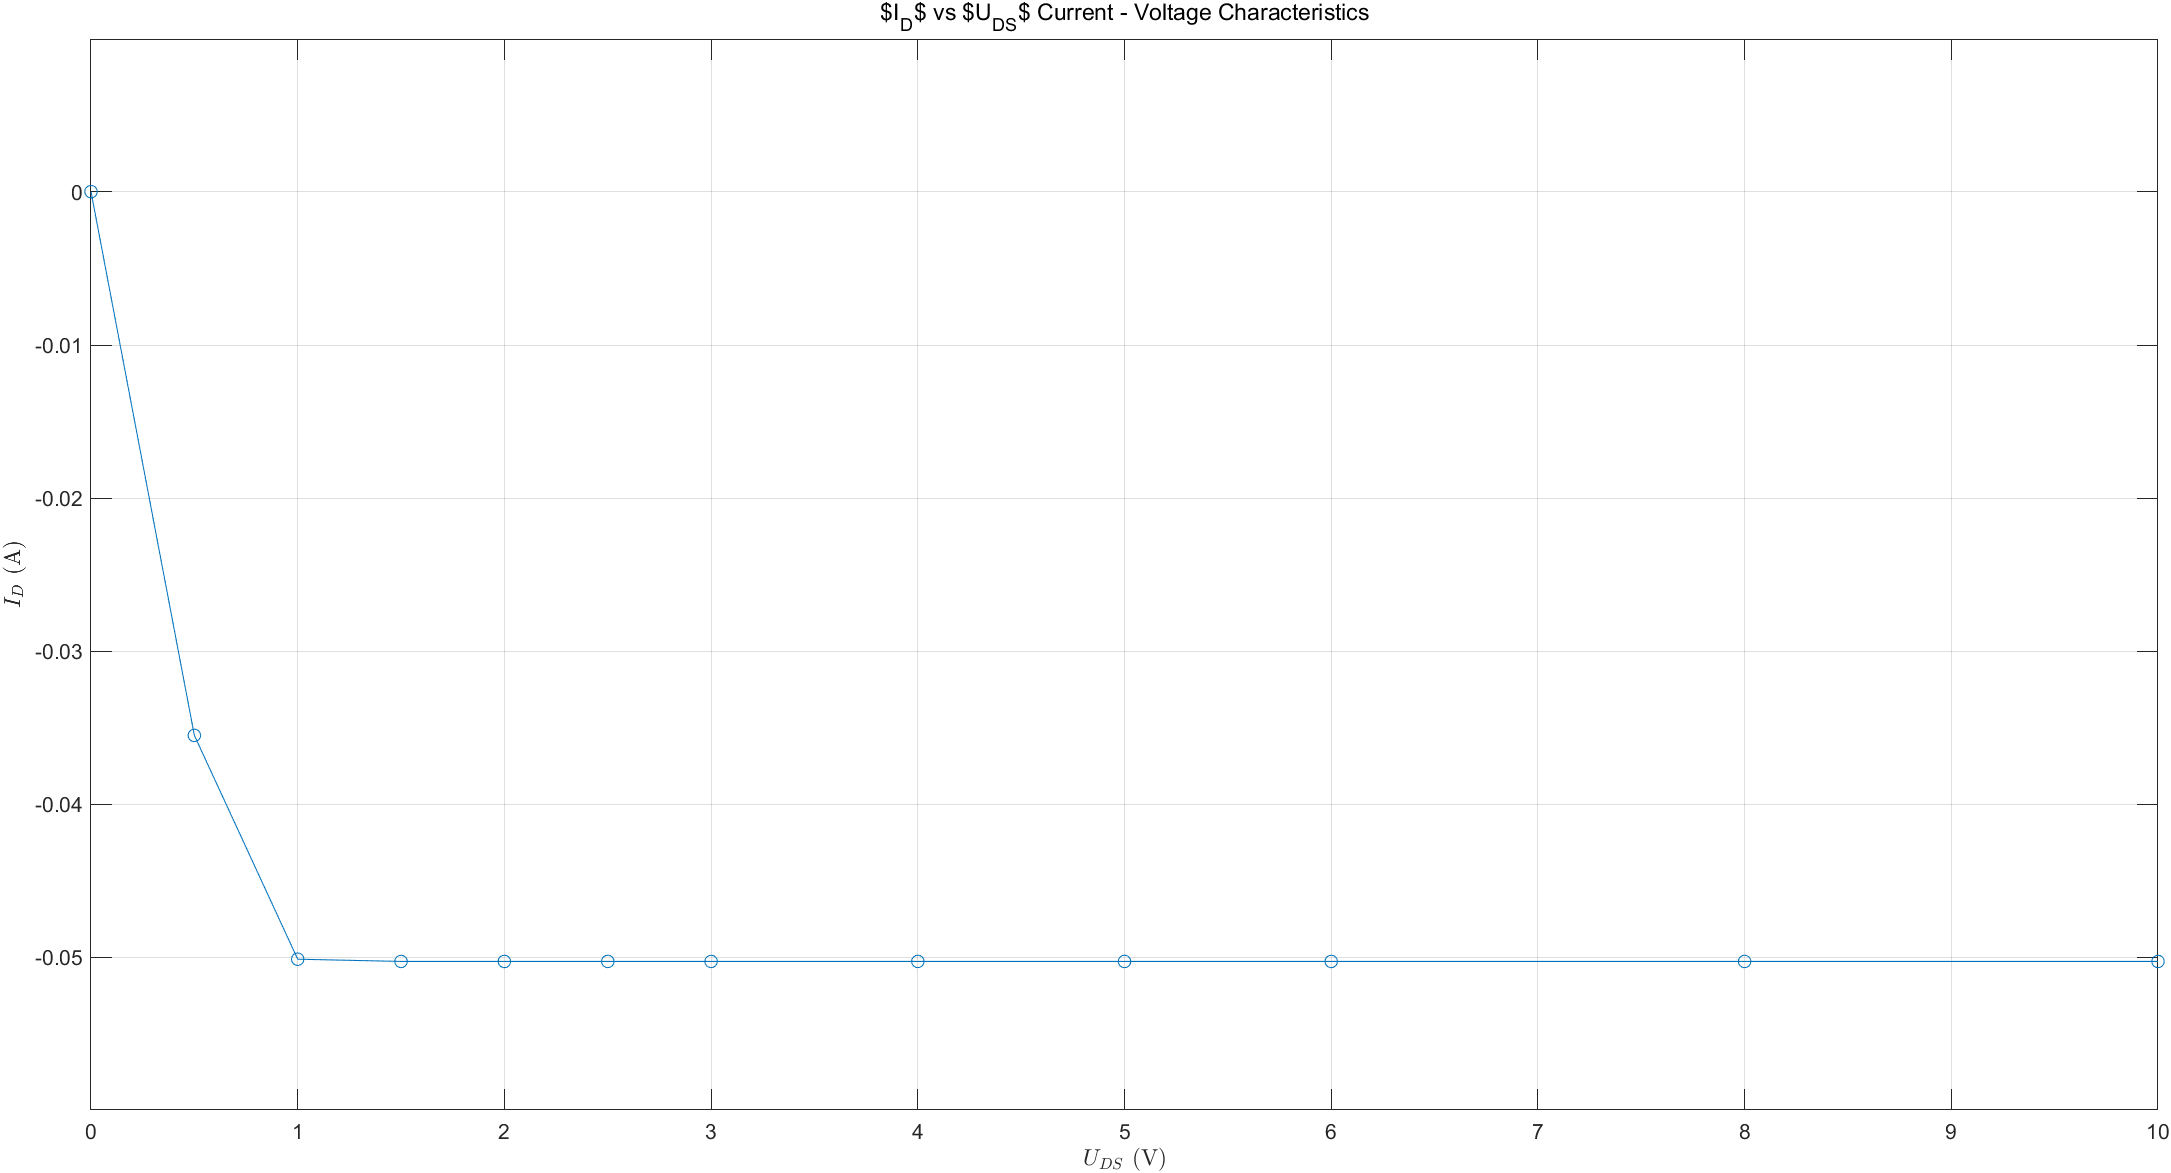
\includegraphics[width=\linewidth]{image/7.png}
        \caption{Id-Uds关系曲线(Ugg=3V)}
        \label{fig:Id-Uds2} 
    \end{minipage}
    
\end{figure}

\newpage

(3)根据前面得到的伏安特性, 分析归纳管子的特点。

开启特性:
随着 $U_{DS}$ 开始增加,电流 $I_{D}$ 迅速变为负值且绝对值增大到一定程度后趋于稳定,这表明在这个 $U_{GS}$一定的条件下(此时$U_{GS}$ 是满足导通条件的,即$U_{GS}$>$U_{GS}$(th)),当 $U_{DS}$ 超过一定阈值后,MOS 管开启,开始有明显的电流流通。

饱和特性:
只要 $U_{GS}$ 保持不变,当 $U_{DS}$ 增大到一定程度后, $I_{D}$ 就不再随 $U_{DS}$ 显著变化。

线性区特性:
在 $U_{GS}$ 满足到导通条件的前提下,当 $U_{DS}$ 处于较低水平(通常 $U_{DS}$<$U_{GS}$−$U_{GS}$(th) )时, 管子工作在线性区。在此区域内,漏极电流 $I_{D}$ 与漏源电压 $U_{DS}$ 近似呈线性关系。此时 MOS 管内部导电沟道完全形成,且沟道电阻相对稳定,随着 $U_{DS}$ 增加, $I_{D}$ 近似线性增大,就如同一个受 $U_{GS}$ 控制的可变电阻 。


\newpage

\section{双极型晶体管(BJT)BJT的特性仿真}
仿真电路如图所示:$R_B = 200K\Omega, R_C = 2K \omega $, 三极管选择2N2222。分别测试在不同$E_b$、$E_c$作用下的三极管电压、电流, 完成下列表格。试画出$I_C$和$U_{CE}$的关系。

\begin{figure}[ht]
    \centering
    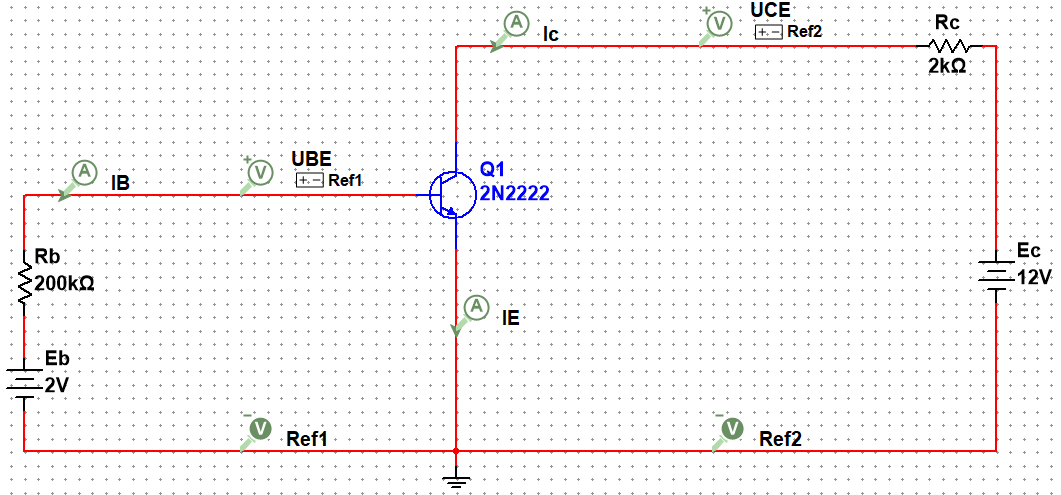
\includegraphics[width=0.8\linewidth]{image/2.png}
    \label{b}
\end{figure}

\begin{table}[ht]
    \centering
    \label{tab:c}
    \begin{tabular}{|c|c|c|c|c|c|}
        \hline
        $E_b(V)$&$E_c(V)$&$U_{BE}(V)$&$I_B(\mu  A)$&$I_C(mA)$&$U_{CE}(V)$\\ \hline
        \multirow{10}{*}{2} &0  &0.51&7.41&0.00&0.00\\ \cline{2-6}
                            &0.5&0.60&6.99&0.19&0.10\\ \cline{2-6}
                            &1  &0.61&6.90&0.42&0.14\\ \cline{2-6}
                            &2  &0.62&6.88&0.59&0.80\\ \cline{2-6}
                            &3  &0.62&6.88&0.67&1.65\\ \cline{2-6}
                            &4  &0.62&6.88&0.74&2.51\\ \cline{2-6}
                            &6  &0.62&6.88&0.89&4.21\\ \cline{2-6}
                            &8  &0.62&6.88&1.03&5.92\\ \cline{2-6}
                            &10 &0.62&6.88&1.18&7.62\\ \cline{2-6}
                            &12 &0.62&6.88&1.33&9.33\\ \hline
        \multirow{10}{*}{4} &0  &0.54&17.29&0.00&0.00\\ \cline{2-6}
                            &0.5&0.60&16.98&0.21&0.07\\ \cline{2-6}
                            &1  &0.62&16.89&0.45&0.09\\ \cline{2-6}
                            &2  &0.63&16.81&0.93&0.12\\ \cline{2-6}
                            &3  &0.64&16.76&1.39&0.20\\ \cline{2-6}
                            &4  &0.64&16.76&1.58&0.83\\ \cline{2-6}
                            &6  &0.64&16.76&1.89&2.20\\ \cline{2-6}
                            &8  &0.64&16.76&2.21&3.56\\ \cline{2-6}
                            &10 &0.64&16.76&2.53&4.93\\ \cline{2-6}
                            &12 &0.64&16.76&2.84&6.30\\ \hline
                    
    \end{tabular}
\end{table}

\newpage
最终画出图像如下:

\begin{figure}[ht]
    \centering
    \begin{minipage}[ht]{0.48\linewidth}
        \centering
        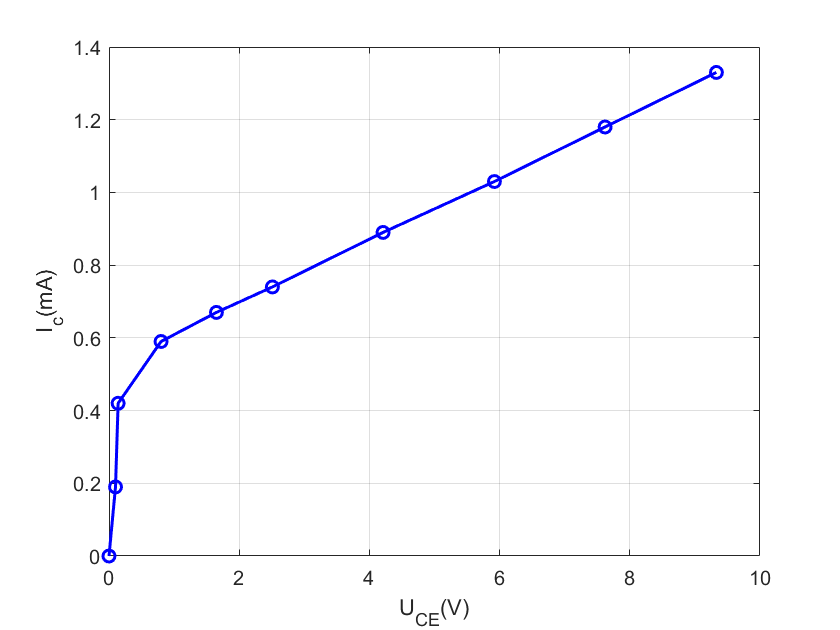
\includegraphics[width=\linewidth]{image/3.png}
        \caption{Ic-Uce关系(Eb=2V)}
        \label{c}
    \end{minipage}
    \hfill
    \begin{minipage}[ht]{0.48\linewidth}
        \centering
        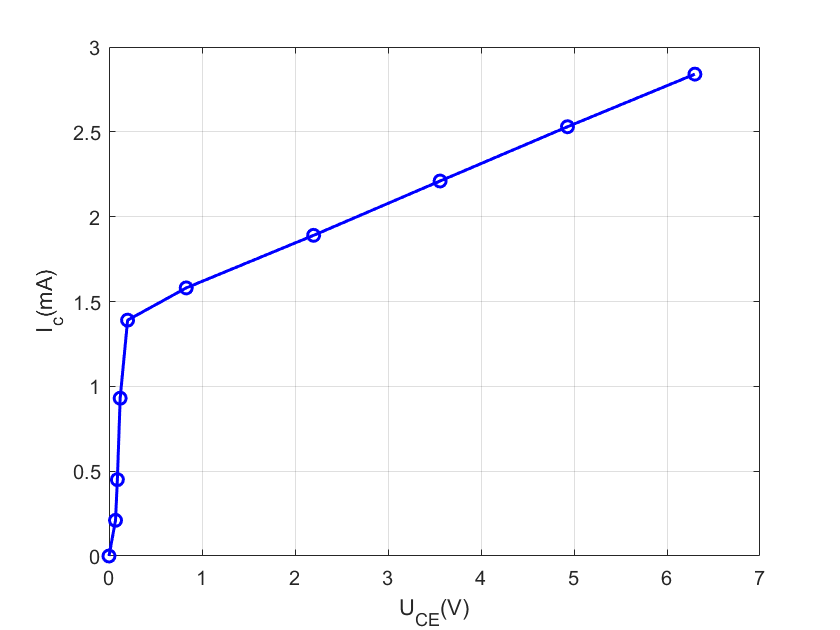
\includegraphics[width=\linewidth]{image/4.png}
        \caption{Ic-Uce关系(Eb=4V)}
        \label{d}
    \end{minipage}
\end{figure}

(1)根据前面得到的伏安特性, 分析归纳管子的特点

管子的开启特性:
随着 $U_{BE}$ 开始增加,电流 $I_{C}$ 迅速变为负值且绝对值增大到一定程度后趋于稳定,这表明在这个 $U_{CE}$一定的条件下(此时$U_{BE}$ 是满足导通条件的,即$U_{BE}$>$U_{BE}$(th)),当 $U_{CE}$ 超过一定阈值后,BJT 管开启,开始有明显的电流流通。

饱和特性:
只要 $U_{BE}$ 保持不变,当 $U_{CE}$ 增大到一定程度后, $I_{C}$ 就不再随 $U_{CE}$ 显著变化。

截止特性:
只要 $U_{BE}$ 保持不变,当 $U_{CE}$ 降到一定程度后, $I_{C}$ 就不再随 $U_{CE}$ 显著变化。此时 BJT 管处于截止状态,几乎没有电流流过。

\section{场效晶体管}
\subsection{工程应用电路}
如图所示
\begin{figure}[ht]
    \centering
    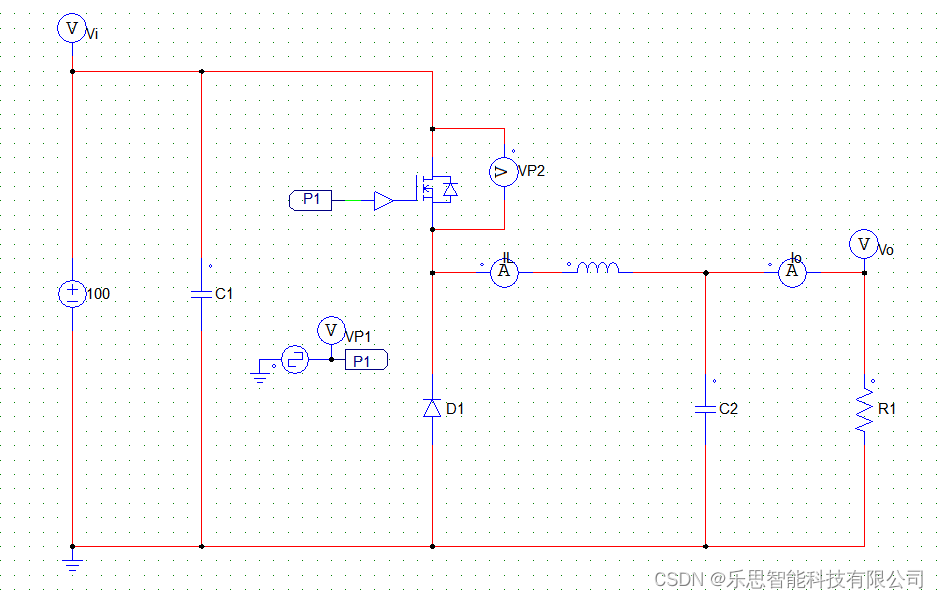
\includegraphics[width=0.8\linewidth]{image/9.png}
    \caption{场效应管buck开关电源电路}
    \label{fig:mosfet_circuit}
\end{figure}
\subsection{功能}
通过MOSFET的开关控制,来实现对负载的电压调节。常见为12V->5V,5V->3V3的降压电源。

\subsection{电路原理}
通过MOSFET的开关,控制电流的通断,从而对电压进行调节,同时应用电容和电感,来平滑电流的波动。
电路中MOSFET的开关频率一般在20KHz-100KHz之间,电感和电容的选择可以根据实际需要进行调整。

\section{BJT管}
\subsection{工程应用电路}
如图所示
\begin{figure}[ht]
    \centering
    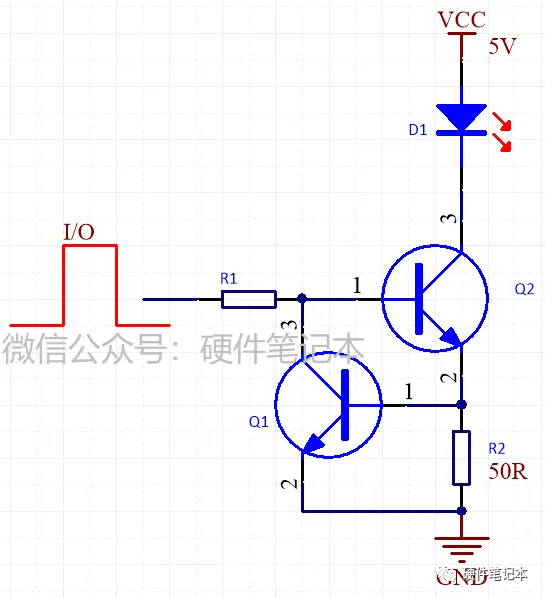
\includegraphics[width=0.8\linewidth]{image/8.png}
    \caption{BJT管恒流源电路}
    \label{fig:bjt_circuit}
\end{figure}

\subsection{功能}
可以为负载提供恒定14mA的电流。

\subsection{电路原理}
电路平衡状态下,由于三极管的基极和发射极之间恒定0.7V压差,使得通路上电流恒定为0.7V/R2 = 14mA。

\end{document}
